
\section{Preface}

This thesis describes some of the research carried out by me and my
colleagues in the \an group.  \an started as a collaboration between
Sam Roweis, a University of Toronto computer scientist, and David
W.~Hogg, a New York University astronomer.  An idea that began as a
crazy scrawl on the back of a napkin---probably in a bar---eventually
grew into a real project and began attracting collaborators and
students.  Fast-forwarding a few years, we have achieved a rare feat:
a computer vision software system that \emph{works}, with little human
intervention, and is being used by hundreds of real astronomers doing
real research.  We have also branched out and explored a number of
other promising areas where ideas in computer vision and machine
learning can be applied to astronomical data to great benefit.


This thesis is quite blatantly a collection of manuscripts.  I have
done a bit more than staple them together to produce the chapters of
this thesis, but the original tone and style of each manuscript still
shines through.  I hope my readers will find the chapter-to-chapter
variations a refreshing, rather than jarring, change of pace.  One
advantage of collecting manuscripts into a thesis is that each chapter
should largely stand alone.  Another advantage is that each manuscript
was prepared with a list of authors, so it is simpler to identify the
collaborators who have contributed to each chapter.


\section{Introduction}


The general idea of the \an collaboration is to apply ideas in
computer vision and machine learning to problems and data in
astronomy.  Astronomical images are a good domain in which to explore
ideas in computer vision, because the problems to be solved are often
much more constrained than in general imaging, the telescopes and
cameras are often well-understood and calibrated, large volumes of
data and ``ground truth'' information exist, and with new telescopes
constantly coming online and producing greater and greater volumes of
imaging, there is a need for sophisticated computation.  I briefly
outline astronomical imaging for computer vision researchers in
\secref{sec:astrointro}.


The specific idea addressed in this thesis is that pattern recognition
approaches can be applied to astronomical images.  The goal is to
produce a system that is able to recognize automatically the stars in
any image of the night sky, using the information in the image pixels
alone.  Recognizing the stars in an image is equivalent to finding the
pointing, scale, and rotation of the image on the sky in a standard
coordinate system.  The branch of astronomy concerned with measuring
the positions and motions of celestial bodies is called
\emph{astrometry}, and the task of placing a new image in a standard
reference frame is known as 
``calibrating the astrometry'' of the image.  The task of calibrating the
astrometry of an image using only the image itself---not given a prior on the
location---was historically known as \emph{blind astrometric calibration}.
We recognize\footnote{Retroactively, in the year 2020}, that this is an
ableist phrase, and instead prefer \emph{full-sky astrometric calibration}.
The broad goal of the \an project was to build a system
that would allow us to create correct, standards-compliant astrometric
\metadata for every useful astronomical image ever taken, past and
future, in any state of archival disarray.  This is part of a larger
effort to organize, annotate and make searchable all the world's
astronomical information.


After a brief introduction to astronomical imaging for computer
scientists, the remainder of this chapter reviews the area of pattern
recognition, and in particular the framework of \emph{geometric
hashing} for object recognition in images.  One of the contributions
of this thesis is to replace the simple hash table used in traditional
geometric hashing with a \kdtree, so I review related work in hashing
and other approaches for fast feature matching.  Finally, I present
the astrometric calibration task as an instance of object
recognition, and review some previous approaches to the problem.

%% Our approach?


The remaining chapters present our approach to the astrometric
calibration problem.  \Chapref{chap:techreport} explains our approach
and presents the results of large-scale tests of the system on
real-world data.  Chapters \ref{chap:verify} and \ref{chap:kdtree}
delve into details of the approach: \Chapref{chap:verify} presents the
Bayesian decision theory problem that lies at the heart of our
approach, while \chapref{chap:kdtree} explains the technical details
of the \kdtree data structure implementation that is key to making our
system fast enough to be a practical tool.
\Chapref{chap:conclusion} summarizes our results.


\section{Astronomical imaging for computer scientists}
\label{sec:astrointro}

Astronomical images are very different from images produced by typical
consumer-grade cameras.  This section is intended to give
non-astronomers a sense of the typical parameters of contemporary
astronomical imaging setups, and introduce some of the terminology and
key ideas.


The Sloan Digital Sky Survey (SDSS) \cite{sdsstechnical, sdsscamera}
is one of the most important projects in contemporary astronomy.  The
primary imaging survey was carried out from 2000 through 2008, so the
hardware is no longer cutting-edge, but it is still very impressive.
The telescope's primary mirror is $2.5$ meters in diameter.  Incoming
light first strikes the primary mirror, then a one-meter secondary
mirror, then passes through two corrective lenses in front of the
camera.  The nearly distortion-free field of view is about $3$ degrees
wide.  The camera is composed of $30$ charge-coupled devices (CCDs),
each $2048\times2048$ pixels, arranged in six columns.  The five CCDs
in each column have different bandpass filters, ranging from the
near-infrared ($913~\nanometers$) through the optical to the
near-ultraviolet ($354~\nanometers$).  The CCDs and associated
electronics are cooled with liquid nitrogen to $-80^{\circ} \unit{C}$
and held under vacuum.  Each CCD is about $5~\unit{cm}$ square, and
the whole focal plane of the camera is about $65~\unit{cm}$ in
diameter.  The camera assembly has a mass over $300~\unit{kg}$.


The survey operates in ``drift-scanning'' mode: the telescope is
pointed in a nearly fixed direction, and as the Earth rotates the sky
drifts past the camera.  The camera electronics shift the electrons
along the CCD columns at the same rate.  As an object drifts through
the field of view, the electrons it produces in the CCD pixels march
along with it, and are read out as it disappears from view.  In the
SDSS camera, the object drifts past each of the five bandpass-filtered
CCDs of the camera in turn, producing a five-color image.  Over the
course of a night of observing, the camera sweeps out a great circle,
creating six columns of five-band images that are $2048$ pixels wide
and over a million pixels long: over $120$ gigabytes of pixels per
night.  This clever drift-scanning scheme has many advantages, one
being that the readout rate of the CCDs can be relatively slow,
resulting in low readout noise.  Calibration of the camera is simpler
because charge is integrated over columns of the CCD: it is only
necessary to calibrate whole columns rather than individual pixels.
Note that for this scheme to work, the CCDs must be very carefully
aligned in the focal plane, and the telescope control system must be
capable of keeping the system pointed stably at the level of a pixel
or better.  The moving mass of the telescope is over
$15,000~\unit{kg}$, so this is no mean feat!

% 24 um pixels

Astronomical imaging systems are designed so that the point-spread
function (PSF)---the image on the CCD of a distant point source of
light---is spread over several pixels.  This allows the position of a
point source to be measured to sub-pixel accuracy by fitting a model
of the PSF to the observed pixel values.  If the system focused a
point source onto a single pixel, this would be impossible.  The goal
is typically for the full-width at half-maximum (FWHM) of the PSF to
be a few pixels, so that the PSF is well-sampled but the signal is not
spread out over too many pixels.

For ground-based telescopes, the moving atmosphere causes the image of
a distant point source of light to dance around on the CCD; in typical
exposures of many seconds this ``speckling'' is integrated into a
point-spread function.  The size of this PSF is called the ``seeing''
and a value of one $\unit{arcsecond}$ FWHM is considered quite good.
The SDSS camera has pixels of size $0.396~\unit{arcseconds}$, and the
point-spread function is dominated by the seeing: the optics of the
system are good enough that the images are as clear as they can be
given the atmosphere.


The positions of astronomical objects are usually measured in an
\emph{equatorial coordinate system}: essentially the projection of the
Earth's latitudes and longitudes onto the celestial sphere at a
specific instant.  The latitudinal direction is called ``declination''
and abbreviated ``Dec'', and the longitudinal direction is called
``right ascension'' and abbreviated ``RA''.  Declination is typically
measured in degrees from $-90$ to $+90$, and right ascension is
typically measured in degrees from $0$ to $360$, or hours from $0$ to
$24$.  There are $60~\unit{arcminutes}$ per degree and
$60~\unit{arcseconds}$ per $\unit{arcminute}$.  For reference, the
Moon as seen from Earth is about half a degree in diameter.  The
$0.396~\unit{arcsecond}$ pixels of the SDSS camera view an area the
size of a penny at a distance of ten kilometers; each $2048\times2048$
pixel CCD views an area of about one-millionth of the sky.


The SDSS is very impressive, but the next generation of telescopes
currently in development dwarf its specifications.  The Large Synoptic
Survey Telescope (LSST) \cite{lsst}, for example, has an
$8.4~\unit{meter}$ primary mirror, with a $3.5~\unit{degree}$ field of
view almost completely covered by an array of nearly $200$ CCDs, each
with $4096\times4096$ pixels: a total of about $3.2$ gigapixels.  The
camera is the size of a small car.  It will take exposures of about
$15$ seconds, yielding over $10$ terabytes of data per night.

% -- basics of data reduction; catalogs
% -- stars, galaxies, and other stuff




\section{Pattern recognition}

\emph{Pattern recognition} encompasses a huge class of problems and
techniques in computer vision and machine learning.  Many pattern
recognition problems are of the type ``identify this object'' or
``find things like this'': the system is first told about a large set
of objects, then is presented with a novel object and is asked to
describe it or find similar objects from the set of known objects.

Pattern recognition systems often take a \emph{feature matching}
approach.  A \emph{feature} is a compact description of
(problem-specific) relevant, invariant properties of an object, such
that objects that are similar in the problem domain have similar
features.  Defining how features are extracted from objects and
defining the similarity between features are key factors in the
success of such systems.  Often the representation of a feature (the
\emph{feature descriptor}) is a point in a real coordinate space and a
distance metric defines the similarity between features.

Feature-based approaches typically involve two phases: an
\emph{indexing} phase, in which the set of known objects is shown to
the system, and a \emph{test} phase, in which novel objects are
presented.  During indexing, features are extracted from the set of
known objects.  At test time, features are extracted from the novel
object and compared with the set of features from the known objects.
In many domains, the set of known objects is very large, so it is
critical that features be stored in a manner that allows the system to
rapidly find known features that match a given feature.

Often feature-based approaches suffer \emph{feature aliasing}
problems: two objects that are dissimilar in the problem domain may
yield similar features.  In this case, systems may use \emph{voting}
or \emph{verification} schemes to ensure that aliased (false) feature
matches are eliminated.  Voting schemes typically assume that false
feature matches are independently randomly distributed, so the
probability of matching several features to the same incorrect object
is the product of the individual probabilities; if we demand a
sufficient number of matches, the probability of a false match becomes
small.  Verification or \emph{hypothesize-test} schemes treat a
feature match as a hypothesis that the novel object is similar to a
known object, and then some test to decide if the hypothesis is
correct.  Such schemes can be seen as using feature matching as a
search heuristic.

\section{Visual pattern recognition}

Pattern recognition in images is a particularly challenging and
complex problem domain which has been studied extensively.  Objects to
recognize include faces, fingerprints, specific physical objects, or
even general classes of physical objects such as mugs, chairs, or
elephants.


Visual pattern recognition of general physical (3-dimensional) objects
is difficult for many reasons: objects may be deformable, can appear
different when viewed from different angles or under different
lighting conditions, and can be occluded by other objects.  Features
used in visual pattern recognition include edges (lines and curves),
corners, or the color or texture of image patches.


An important consideration when designing features for visual pattern
recognition is the size (\ie, spatial extent in the image) of the
feature.  \emph{Local features} gather information from a small region
of the image, while \emph{global features} incorporate information
from the whole image.  Local features can provide robustness to
occlusion and deformation: if part of the object is hidden, features
belonging to that part will be lost, but the features belonging to the
remaining parts will still be found.  Since local features aggregate
information from only a small portion of the image, they may be more
noisy or less distinctive than global features.


Since a single local feature may be insufficient to guarantee that an
object has been correctly recognized, some systems build high-level
features by combining multiple low-level features.  When the objects
to be recognized are rigid or articulated (composed of multiple rigid
parts connected by simple joints), a common approach is to build
features that describe the relative geometry of low-level features.
This use of \emph{geometric features} is often called \emph{geometric
hashing}, since the result is a feature descriptor or \emph{hash code}
which describes the geometric arrangement of the low-level features.



\section{The geometric hashing framework}

\begin{figure}
\begin{center}
% dot lamdan.dot -Tps2 -o lamdan.ps
% ps2pdf -sPAPERSIZE=a4 lamdan.ps lamdan.pdf
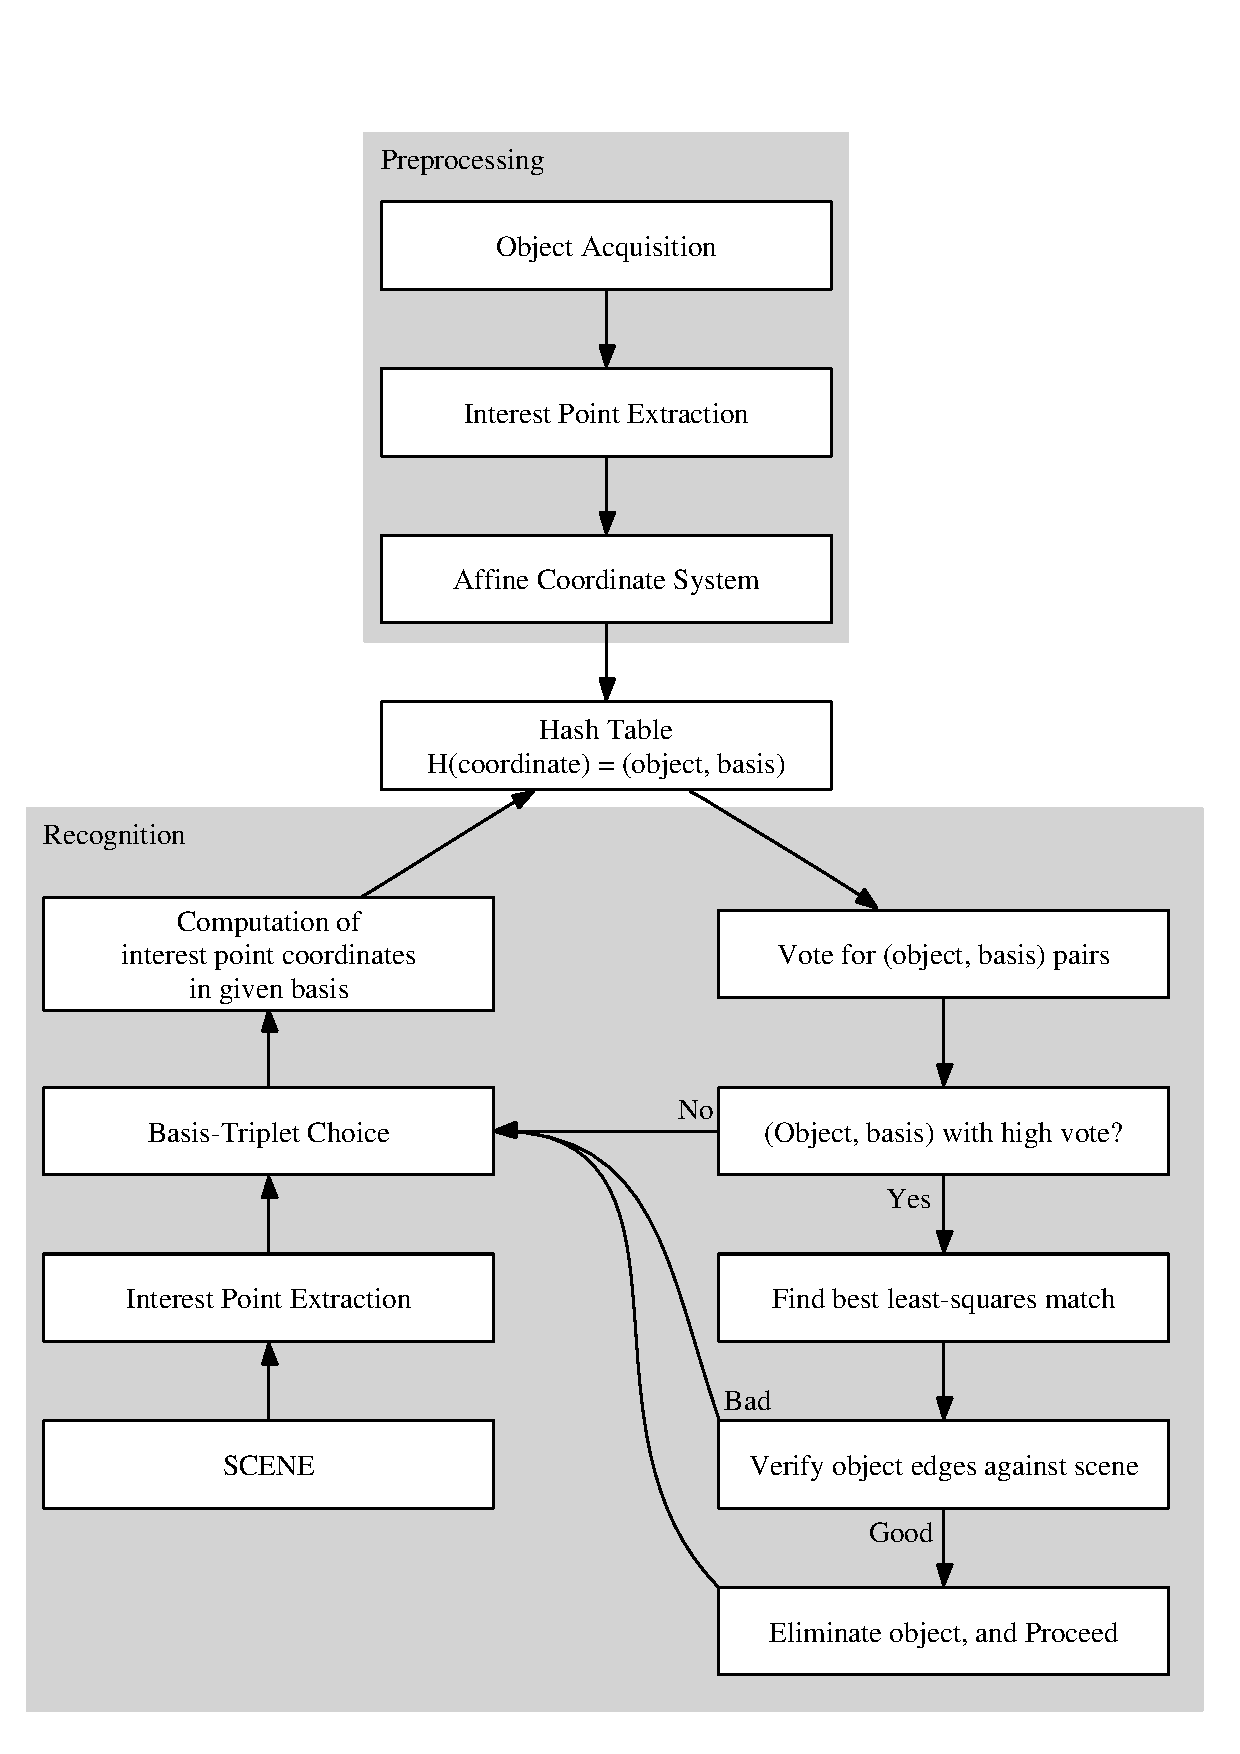
\includegraphics[height=0.8\textheight]{lamdan}
\end{center}
\caption{Outline of the Geometric Hashing scheme.  This diagram is a
  reproduction of \fig 2 in Lamdan \etal \cite{lamdan1990}.
  \label{lamdan}}
\end{figure}


Lamdan \etal \cite{lamdan1990} and Wolfson and Rigoutsos
\cite{wolfson1997} give an excellent overview of the geometric hashing
approach.  See Figure \ref{lamdan} for a block-diagram overview.
Geometric hashing is based on the fact that when rigid objects undergo
similarity transformations (translation, rotation, and scaling),
angles between points on the object and relative distances between
points do not change.  Therefore, if we describe the relative
arrangement of points on an object in terms of these invariants, our
description will be invariant under these transformations of the
object.  Invariant geometric properties can be found for other types
of transformations such as affine or perspective projection.


Geometric hashing builds \emph{geometric features} out of lower-level
features.  We will call the low-level features \emph{interest points}
for clarity.


Given the types of transformations the system must handle, there is
some sufficient number of interest points required to define an
invariant local coordinate system; these are called the \emph{basis
  set}.  For example, for 2-D objects that can undergo similarity
transformations, two interest points can be used to define a
coordinate system.  For 3-D objects with similarity transformations,
three (non-collinear) interest points are required.

Geometric hashing follows an indexing approach.  During the indexing
phase, the system preprocesses a database of objects which are to be
recognized.  For each object, many interest points are extracted which
are invariant under the transformations that are expected, and can be
well localized.  The system then enumerates all basis sets by looking
at all combinations of interest points; each set of basis features
defines a relative coordinate system.  For each basis set, all
remaining interest points are enumerated and their positions described
in this coordinate system.  Each relative coordinate vector forms a
\emph{geometric feature descriptor}.  In this way, the relative
geometric arrangement of a set of interest points is converted into a
point in a vector space.

% --- consider adding a variant of the quad fig here.

In the standard geometric hashing approach, the geometric feature
descriptor is discretized and encoded as a hash table key. A grid is
placed over the feature descriptor space, and the hash table key of a
geometric feature is the identifier of the grid cell containing it.
Each entry in the hash table maps back to the basis set plus the
feature whose position is encoded.

% --- picture?

Given a new image, a geometric hashing system extracts all interest
points from the image and, as at indexing time, proceeds to enumerate
all basis sets and computes the positions of the remaining interest
points in each basis set.  This generates many geometric features
whose descriptors are discretized and converted to hash table keys, as
before.  Similar arrangements of interest points will lead to similar
geometric feature descriptors, which--with luck---will be mapped to
the same hash table key.  The hash table values associated with each
key are retrieved, and each value that is found is considered a match.
Each match votes for the correspondence between the interest points
from the database and the interest points from the image that were
used to define the geometric feature.


After all features from the image have been processed, many votes will
have accumulated.  False matches (due to aliasing or hash table
collisions) should be uniformly distributed over the set of known
objects, so should not generate very many votes for any particular
object.  Objects that are actually present in the image should
generate many votes.  Objects that receive an insufficient number of
votes are rejected, and the remainder are subjected to a verification
process.


The verification process requires computing a transformation from the
object to image coordinates, using the corresponding interest points
from the known object and the image.  Using this transformation, all
the interest points belonging to the known object are projected into
image coordinates.  If the match is correct, we expect the image to
contain features at these locations.  Some researchers add an extra
verification stage by projecting the known object into the image and
checking that the predicted edges of the object are found in the image
(eg, \cite{lamdan1990, huttenlocher1990}).


The geometric hashing approach is flexible and applicable to many
problems, but there are some issues with the basic version described
here.  The hash function described above simply places a grid over the
relative coordinate system and returns the identifier of the grid cell
in which the interest point lands.  This is prone to edge effects: if
an interest point is near the edge of a grid cell, a small change in
its position due to noise can move it across the edge into a different
grid cell, which causes the hash code to change and a different set of
feature matches to be found.  This problem can be overcome by
detecting interest points that are near the edges of their cells and
also searching the hash table using the hash codes of neighbouring
cells.  This results in more false feature matches, and can become
expensive as the dimensionality of the geometric feature space
increases (there are more edges, and the proportion of the hypervolume
of feature space that is near an edge increases).  Using a data
structure other than the hash table may be beneficial.


Another issue with uniform grid-based hashing is that it assigns equal
importance (and storage space) to each grid cell in the feature space.
Consider an interest point that is far from the basis set that defines
its local coordinate system.  Small positional errors in the basis set
can cause the coordinate system to be rotated or scaled, which results
in large changes in the interest point's relative coordinates.  This
means that edge effects become more pronounced in such regions of the
feature space.  One response to this concern is to increases the size
of the grid cells far from the basis set, but then if the interest
points are uniformly distributed, these larger hash table bins will
contain more features, so every match to these bins will be
accompanied by more false positives.


Finally, a hash table with equal-sized cells will only be uniformly
utilized if interest points are uniformly distributed in feature
space, but some domains may yield interest points that are far from
uniformly distributed.  In other domains, it may be beneficial to
place constraints on the geometric features that are used (for
example, to avoid regions that are prone to large errors, or that are
relatively indistinctive).


There is nothing in the geometric hashing framework that requires a
standard hash table to be used for feature matching.  Other methods of
feature matching are described in the next section.


\section{Related work in fast feature matching}


For feature matching in a geometric hashing framework, the database of
known objects is converted into a set of points in a feature
descriptor space, which is a vector space.  To find matches to a new
feature (extracted from an image in which we want to recognize
objects), we need to find all points in the vector space that are
within some tolerance.  Usually the Euclidean distance metric is
applied, so the tolerance is a radius in the vector space.


\subsection{Bloom filters}

A Bloom filter \cite{bloom1970} is a data structure that can answer
queries of the form ``is feature $q$ a member of the set of known
features?''  A Bloom filter is a set of $n$ bits, initially zero.  A
set of $k$ hash functions must be defined which take a feature as
input and produce an integer in $[0, n)$ as output.  In the indexing
phase, we examine each of the known features, and apply each of the
hash functions, producing $k$ hash codes.  Each code is used to
reference a bit and \emph{set} it (\ie, turn it on).  Each known
feature results in $k$ bits being set; several features may request
that a particular bit be set.


Given a new feature to match, we run the $k$ hash functions on it and
test whether each of the resulting bits are set.  If the feature is
equal to a feature seen at indexing time (according to the hash
functions), then all $k$ of the bits will have been set; thus the
Bloom filter does not produce false negatives.  If the query feature
is not equal to a known feature, then some of the bits may have been
set due to \emph{collision} of the hash functions, but the feature
will only be accepted if all $k$ hash functions result in collision;
this results in a false positive.  The rate of false positives
increases as the number of known features increases relative to the
number of bits in the filter.  The Bloom filter is ideally suited to
cases where the number of known features is small, and a verification
step can be applied to eliminate any false positives that are
produced.


For feature matching, we want to know not only whether the query
feature $q$ matches a known feature, we want to know \emph{which}
known feature matches.  One way to answer such queries is to use a
\emph{Bloomier filter} \cite{chazelle2004}.  The simplest Bloomier
filter uses multiple Bloom filters to categorize a given feature into
two different categories, and uses slightly more space than two Bloom
filters.  A set of $n$ such Bloomier filters can be used to categorize
a feature into $2^n$ different categories by assigning one Bloomier
filter to each bit of the result.


The standard Bloom filter only finds exact matches, but we want to
find \emph{nearby} matches.  An extension of Bloom filters to allow
proximity searches is given by Kirsch and Mitzenmacher
\cite{kirsch2006b}.  This variant uses \emph{locality sensitive
hashing} (LSH, discussed below) as its hashing function, so it
inherits some limitations from LSH.  Most importantly, LSH only
guarantees with some probability that nearby features will hash to the
same bin.  As a result, the locality-sensitive Bloom filter can
produce false negatives as well as false positives.


In order to answer feature matching queries (find all known features
near a given query feature), one could combine these Bloom filter
extensions to build a locality-sensitive Bloomier filter.  However,
the false negative rate of the locality-sensitive filter would be
magnified because the Bloomier filter requires \mbox{$2
\ceil{\log(n)}$} separate filters to represent $n$ known features, and
all of these filters must produce the correct answer.  It seems that
Bloom filters are not particularly well suited to this task.


\subsection{Locality Sensitive Hashing}

Locality Sensitive Hashing (LSH) \cite{datar2004, gionis1999,
andoni2006}, is a technique for answering approximate nearest
neighbour queries: it returns a feature whose distance is within a
constant factor of the distance to the nearest neighbour.  The LSH
scheme can be extended to handle exact nearest-neighbour queries
efficiently if the set of known features satisfies some \emph{bounded
growth} criteria.  It is intended for use in high-dimensional spaces
(tens to thousands of dimensions), and $\ell_p$ distance metrics for
$p \in (0, 2]$.


The core idea of LSH is to use several hash functions with the
property that the probability of collision---features being placed in
the same bin---is much higher for nearby features than for distant
ones.  In the indexing stage, we populate the hash table by running
each hash function on each known feature.  To perform a query, we run
the hash functions on the query feature and retrieve the features in
the same hash table bin as the query.  One of these features is likely
to be an approximate nearest neighbour of the query.


In practice, in \cite{datar2004} each hash function is composed of
several (typically $10$) simpler hash functions.  Each simple hash
function performs a random projection in the feature space: the hash
value is the discretized value of the dot product of the feature
vector with the hash function's random vector.  Combining several of
these simple hash functions is equivalent to projecting the feature
vectors onto a grid in a $10$-dimensional, non-orthogonal, subspace.
The hash code is simply the identifier of the grid cell in which the
feature falls.


This scheme suffers from edge effects: a query feature may land in a
bin other than the bin containing its nearest neighbour due to small
positional noise in any of the dimensions.  Attempting to reduce this
effect by making the bin size (discretization level) larger fails
because the number of hash functions must be increased to maintain the
same total number of hash bins.


In order to reduce the number of false negatives, we can choose many
(typically $30$) different hash functions and place a reference to
each feature in the hash table bin chosen by each function.  This
increases the probability that at least one of the hash functions will
select a $10$-dimensional subspace in which the query is close to its
nearest neighbour.


The standard LSH scheme does not seem particularly well suited for the
purpose of feature matching in a geometric hashing system, since the
dimensionality of the feature vectors is usually moderate ($2$ to $6$
in the \an system). Since some feature aliasing is expected in
geometric hashing systems, the nearest neighbour may not be the
correct match: we would prefer to get all neighbours within a given
search radius.


\subsection{\Kdtrees}

\begin{figure}
  \begin{center}
	% tree-figs.py : plot_bboxes
    \begin{tabular}{c@{\hspace{3pt}}c@{\hspace{3pt}}c}
      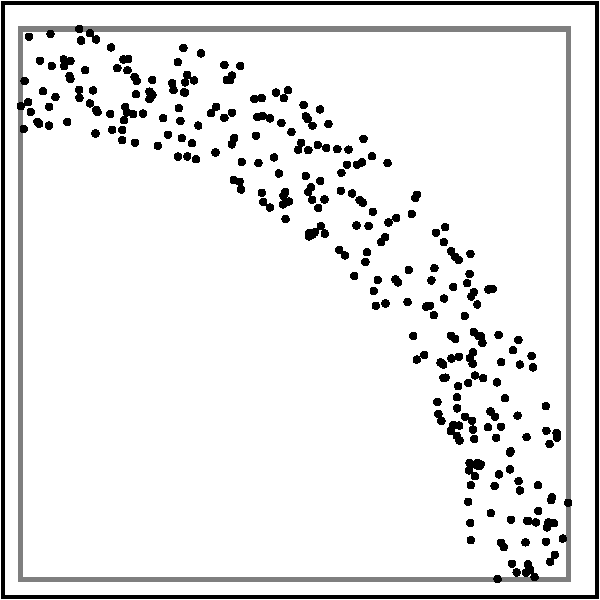
\includegraphics[width=0.31\textwidth]{kdtree-0} &
      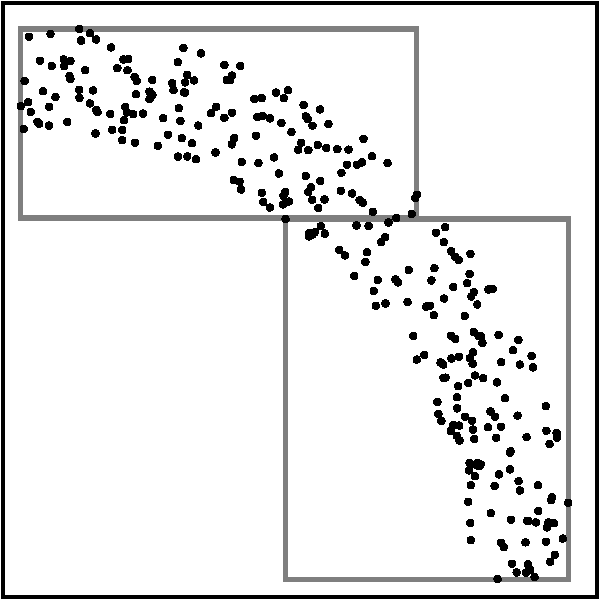
\includegraphics[width=0.31\textwidth]{kdtree-1} &
      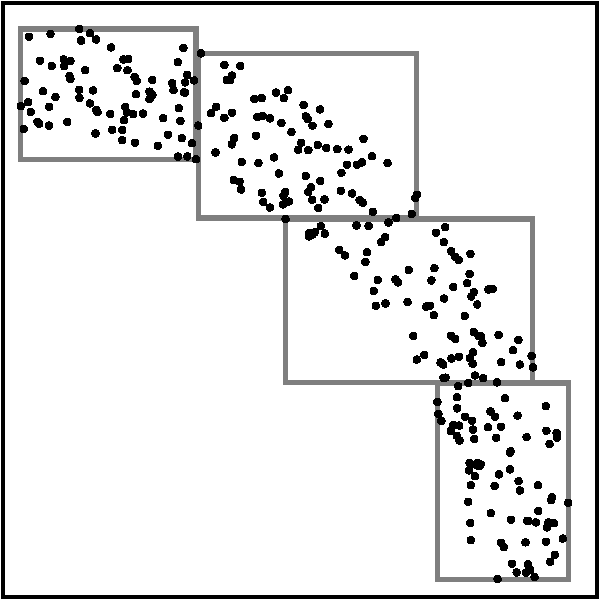
\includegraphics[width=0.31\textwidth]{kdtree-2} \\
      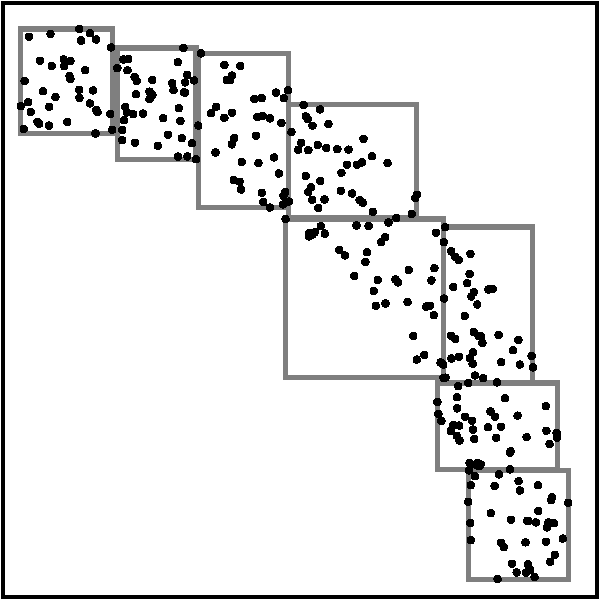
\includegraphics[width=0.31\textwidth]{kdtree-3} &
      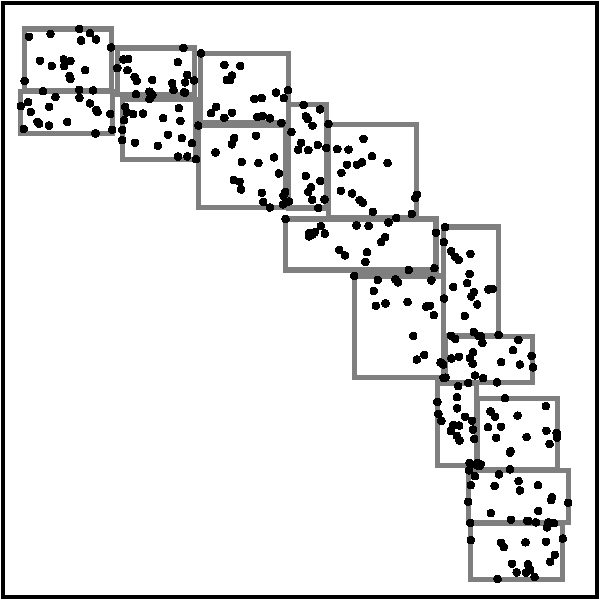
\includegraphics[width=0.31\textwidth]{kdtree-4} &
      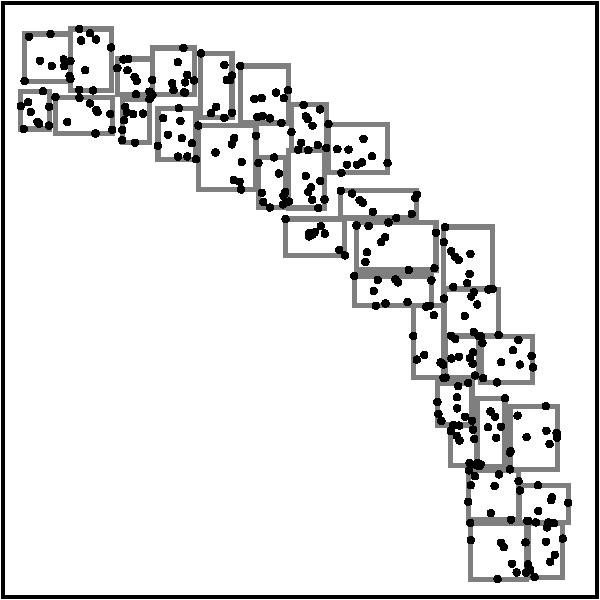
\includegraphics[width=0.31\textwidth]{kdtree-5}
    \end{tabular}
  \end{center}
  \caption[A \kdtree partitioning of space.]{A \kdtree partitioning of
	space.  Each panel shows the nodes at one level of the tree.  The
	points are 200 samples from a ring with uniformly-distributed
	radius in $\left(0.8, 1\right)$ and uniformly-distributed angle in
	$\left(0, \displaystyle{\frac{\pi}{2}}\right)$.  Nodes are split
	along the dimension with the largest range, and the splitting
	position is chosen so that the two child nodes will contain an
	equal number of points.  Note how the tree adapts to the
	distribution of the data: each node tightly bounds the data points
	it owns.  This is a slightly different version of the \kdtree than
	Bentley's original description.\label{kdtree}}
\end{figure}

The $k$-dimensional tree (\kdtree) was introduced by Bentley in 1975
\cite{bentley1975}, and several extensions have been described
\cite{friedman1977, sproull1991}.  The idea is to build a binary tree
over the feature space, where each node ``owns'' a region of the space
which is disjoint from the region owned by its sibling node.  Each
non-leaf node has an axis-aligned splitting hyper-plane; its left
child owns the subspace to the left of the splitting plane, and the
right child the subspace to the right.  In this way, the \kdtree
defines a hierarchical subdivision of the feature space into
axis-aligned hyper-rectangles.  See \figref{kdtree}.


For the purposes of indexing the features in a geometric hashing
system, the set of features is known beforehand and is static, so we
do not need to insert or delete features from the tree, and Bentley's
\emph{optimized} \kdtree construction method can be used.  That is,
the tree can be built to adapt to the particular set of features we
have.


Tree construction proceeds by first assigning all features to the root
node, then recursively splitting nodes until each leaf node owns at
most $L$ features, with $L$ perhaps $10$ or $20$.  Splitting is done
by selecting a splitting plane and using it to partition the features.
Sproull \cite{sproull1991} enumerates several strategies for choosing
the splitting hyperplane.  Traditionally, \kdtrees use axis-aligned
splitting hyperplanes, and the splitting dimension is chosen by simply
iterating through the dimensions (as in Bentley's original paper), or
by selecting the dimension with the largest \emph{range} or
\emph{variance}.  One can also use an arbitrary splitting hyperplane,
for example by finding the principal eigenvector of the covariance
matrix of the feature vectors.  Typically the splitting hyperplane is
positioned so that the two children own an equal number of data
points.  This leads to a balanced (and therefore short) tree, but in
some applications it can be beneficial to bias the splitting location
\cite{macdonald1990}.


Depending on the application, it can be beneficial to store at each
node the tight axis-aligned bounding box (and other summary statistics
\cite{deng1995}) of the points owned by that node (as shown in
\figref{kdtree}).  This is particularly useful where there is
significant correlation between the dimensions of the data, because
splitting the data points along one dimension implies that the
bounding box will shrink in other dimensions as well, and this can
result in faster searches.  If the bounding boxes are stored, then it
is no longer strictly necessary to store the splitting hyperplane,
though it may be useful to speed up some computations.


For feature matching, we typically want to do \emph{range search}:
find all features within radius $r$ of a given query feature $q$.
This is easily achieved with a \kdtree using a recursive algorithm.
Starting at the root, we must decide whether we need to recurse on
each of the node's children.  (How we make this decision is explained
below.)  Once we reach a leaf, we enumerate the features owned by the
leaf and compute the distance to the query feature; any feature with
distance less than $r$ is accepted.


We decide whether we must recurse on a node's children based on their
bounding boxes.  We compute the \emph{mindist}---the lower-bound of
distance---between the query point and each child's bounding box.  The
mindist is simply the distance to the corner or edge of the bounding
box, and can be computed quickly.  Any node whose mindist to the query
point is less than the query radius $r$ must be visited.  If the
\kdtree does not explicitly store the tight bounding-boxes of the
nodes, loose bounding-boxes can be constructed during the recursion
based on the splitting planes of the ancestors.


Chapter \ref{chap:kdtree} presents the \kdtree in more detail.


\subsection{Other approaches}

% Voronoi:
% -de Berg 1997
%   (Mark de Berg , Marc van Kreveld , Mark Overmars , Otfried Schwarzkopf, Computational geometry: algorithms and applications, Springer-Verlag New York, Inc., Secaucus, NJ, 1997)
% -Edelsbrunner 1987
%   (Herbert Edelsbrunner, Algorithms in combinatorial geometry, Springer-Verlag New York, Inc., New York, NY, 1987)
% -Preparata and Shamon 1985
%   (Franco P. Preparata , Michael I. Shamos, Computational geometry: an introduction, Springer-Verlag New York, Inc., New York, NY, 1985)

In contrast to the \kdtree's rectangular decomposition of space, there
is a family of space decompositions that use hyperspheres.  An example
is the \emph{ball-tree} \cite{uhlmann1991b}, in which each non-leaf
node is associated with one of the known features $f$ and a radius
$r$; the left child owns all features within radius $r$ of feature
$f$, and the right child owns the remaining features.  Similarly, in
the \emph{anchors hierarchy} \cite{moore2000}, each non-leaf node is
represented by a feature (called its \emph{anchor}), and a node owns
all the features that are closer to its anchor than the anchor of its
sibling.  These sphere-based trees are supposed to better capture the
structure of high-dimensional data sets, though the results seem to
depend quite strongly on the particular data distributions and search
parameters.


For two-dimensional feature spaces, algorithms based on planar point
location (eg, \cite{kirkpatrick1983}) and the Voronoi tesselation of
space yield $\mathcal{O}(n \log n)$ preprocessing time, a data
structure of size $\mathcal{O}(n)$, and query time of
$\mathcal{O}(\log{n})$.  Unfortunately, in higher dimensions the space
required to store the Voronoi tesselation is
$\mathcal{O}(n^{\floor{d/2}})$, which quickly becomes untenable
\cite{arya1998}.

% planar point location:
% -Dobkin and Lipton in 1976 O((log n)^2) time, O(n^2) space
% -Sarnak and Tarjan O(n) space, O(log n) time
%    * Neil Sarnak, Robert E. Tarjan (1986). "Planar Point Location Using Persistent Search Trees". Communications of the ACM 29 (7): 669-679. 
% -Edelsbrunner, Guibas, and Stolfi, same
%    * Herbert Edelsbrunner, Leonidas J. Guibas, Jorge Stolfi (1986). "Optimal point location in a monotone subdivision". SIAM Journal on Computing 15 (2): 317-340. 
% -Kirkpatrick, same
%    * David G. Kirkpatrick (1983). "Optimal Search in Planar Subdivisions". SIAM J. Comput. 12: 28-35. 
% Voronoi tesselation:
% -B. Delaunay, Sur la sph�re vide, Izvestia Akademii Nauk SSSR, Otdelenie Matematicheskikh i Estestvennykh Nauk, 7:793-800, 1934

The design of spatial indexing data structures and search algorithms
is itself a large research area.  Dozens of different tree structures
have been proposed: in two surveys B\"ohm \cite{bohm2001} and
Hjaltason \cite{hjaltason2003} identify B-, $\textrm{B}^{+}$-, ball-,
bisector-, BSP-, DABS-, fq-, gh-, \mbox{GNA-,} hB-, $\textrm{hB}^{\pi}$-,
hybrid-, IQ-, kd-, kd-B-, $\textrm{LSD}^h$-, M-, mb-,
$\textrm{mb}^{\ast}$-, mvp-, oct-, \mbox{post-office-,} pyramid-, quad-, R-,
$\textrm{R}^{\ast}$-, $\textrm{R}^{+}$-, sa-, slim-, \mbox{sphere-,}
SR-, SS-, TV-, vp-, $\textrm{vp}^{\ast}$-, and X-trees.  There is an
equally mind-boggling variety of exact and approximate search
algorithms.  Each data structure and algorithm may work well in some
region of parameter space, but there is no clear winner for
general-purpose use.


\section{Astrometric calibration as a pattern recognition task}


\comment{
wget "http://casjobs.sdss.org/ImgCutoutDR7/getjpeg.aspx?ra=166.45&dec=-0.03&scale=1&opt=&width=2000&height=2000" -O ngc3521-orig.jpg
jpegtopnm ngc3521-orig.jpg | pnmrotate -45 | pnmcut 600 900 1400 1000 | pnmscale -reduce 2 | pnmtojpeg > ngc3521.jpg
#---> http://live.astrometry.net/status.php?job=alpha-200906-68444159
jpegtopnm ngc3521.jpg | ppmtopgm | pnminvert | pnmtojpeg > ngc3521-bw.jpg
#---> http://live.astrometry.net/status.php?job=alpha-200906-36181848

plotstuff -W 700 -H 500 -J -o ngc3521-sources.pdf < ngc3521-sources.plot
plotstuff -W 700 -H 500 -J -o ngc3521-index.pdf   < ngc3521-index.plot
(at rev 13653)

%%% scp gmaps:/data2/test-merc/tycho.mkdt.fits .
wget "http://explore.astrometry.net/tile/get/?layers=tycho,grid,userboundary&arcsinh&wcsfn=alpha/200906/36181848/wcs.fits&gain=-0.5&bb=0,-85,360,85&dashbox=0.1&w=500&h=500&lw=3" -O ngc3521-zoom0.png
wget "http://explore.astrometry.net/tile/get/?layers=tycho,grid,userboundary&arcsinh&wcsfn=alpha/200906/36181848/wcs.fits&gain=-1&bb=175.533,-17.7621663832,211.533,17.6598478619&dashbox=0.01&w=500&h=500&lw=3" -O ngc3521-zoom1.png
wget "http://explore.astrometry.net/tile/get/?layers=tycho,grid,userboundary&arcsinh&wcsfn=alpha/200906/36181848/wcs.fits&gain=0.5&bb=191.733,-1.85338140354,195.333,1.74602498613&w=500&h=500&lw=3" -O ngc3521-zoom2.png
for x in 0 1 2; do
 pngtopnm ngc3521-zoom${x}.png | ppmtopgm | pnminvert | pnmtopng > ngc3521-zoom${x}-bw.png;
done
}

% ~/an-2/usnob-map/execs/tilerender -x 0.000000 -y -85.000000 -X 360.000000 -Y 85.000000 -w 1024 -h 1024 -l 'tycho' -l 'grid' -l 'boundary' -s -g -0.5 -W 'tor/200706/51145570/wcs.fits' -L 5 -B 0.1 -d > tile1.png
% ~/an-2/usnob-map/execs/tilerender -x 151.724000 -y -4.784223 -X 187.724000 -Y 29.772221 -w 1024 -h 1024 -l 'tycho' -l 'grid' -l 'boundary' -s -g -0.25 -W 'tor/200706/51145570/wcs.fits' -L 5 -B 0.01 -d > tile2.png
% ~/an-2/usnob-map/execs/tilerender -x 167.924000 -y 11.335527 -X 171.524000 -Y 14.841399 -w 1024 -h 1024 -l 'tycho' -l 'grid' -l 'boundary' -s -g 0.5 -W 'tor/200706/51145570/wcs.fits' -L 5 > tile3.png
%
% /home/gmaps/an-2/quads/plotxy2 -i /home/gmaps/ontheweb-data/tor/200706/51145570/index.xy.fits -S 1 -W 720 -H 503 -x 1 -y 1 -w 2 -r 6 -s s > ixy.pgm
% /home/gmaps/an-2/quads/plotxy2 -i /home/gmaps/ontheweb-data/tor/200706/51145570/field.xy.fits -S 1 -W 720 -H 503 -r 5 -x 1 -y 1 -w 2 -s c > fxy.pgm
% cp /home/gmaps/ontheweb-data/tor/200706/51145570/image.pnm undim.ppm
% pgmtoppm green ixy.pgm > ixy.ppm
% pnmcomp -alpha=ixy.pgm ixy.ppm undim.ppm > sum.ppm
% pnmcomp -alpha=fxy.pgm fxy.ppm sum.ppm > sum2.ppm
% pnmtopng sum2.ppm > sum.png
% pnmcomp -alpha=fxy.pgm fxy.ppm undim.ppm | pnmtopng > sources.png
% http://oven.cosmo.fas.nyu.edu/test/status.php?job=tor-200706-51145570


\begin{figure}
\begin{center}
\setlength{\fboxsep}{0.5pt}
\framebox{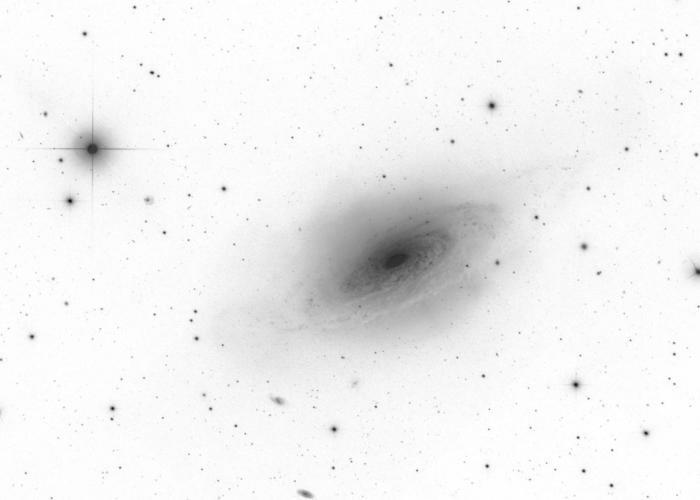
\includegraphics[width=0.99\figunit]{ngc3521-bw}} \\
\framebox{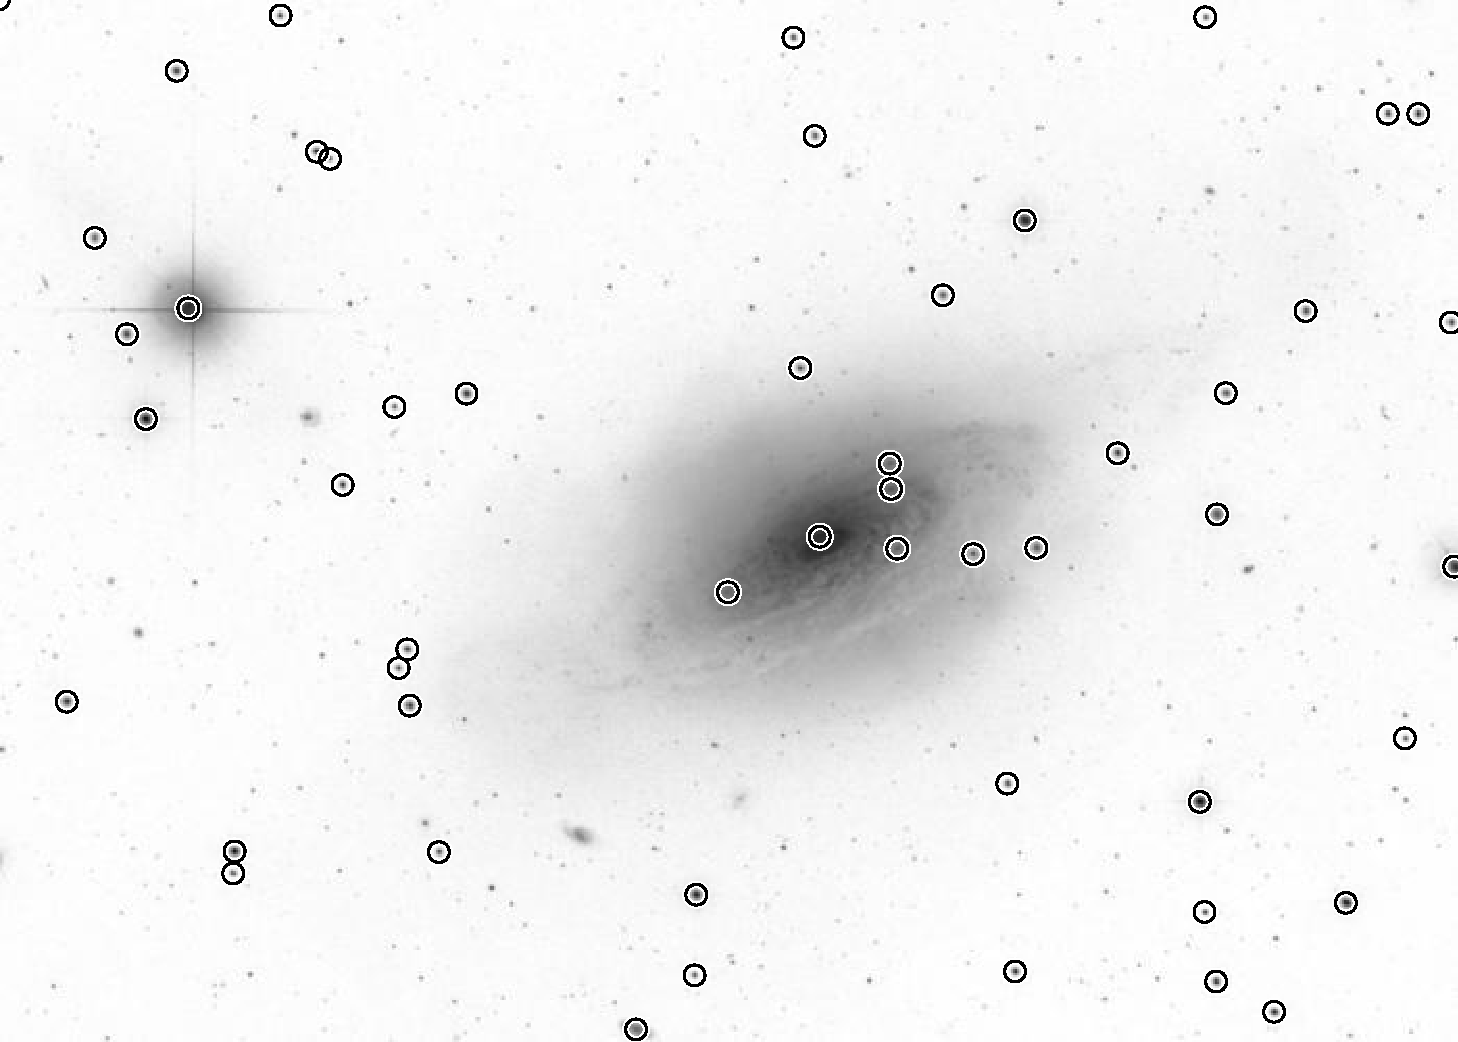
\includegraphics[width=0.99\figunit]{ngc3521-sources}} \\
\framebox{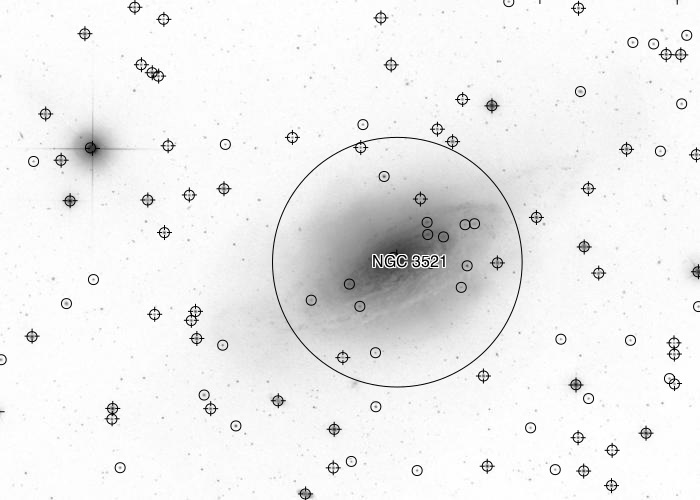
\includegraphics[width=0.99\figunit]{ngc3521-index}}
\end{center}
\caption{\captionpart{Top:} Input image (credit: Sloan Digital Sky
Survey).  \captionpart{Middle:} The brightest 100 sources extracted
from the image.  \captionpart{Bottom:} Reference sources, transformed
into the image coordinate system (crosshairs).  Many of the image and
reference sources are aligned, but there are many image sources
without reference sources.  Our system knows about the positions of
many objects of interest on the sky, and has labelled the galaxy NGC
3521.\label{fig:redgreen}}
\end{figure}


\begin{figure}
\begin{center}
\setlength{\fboxsep}{0.5pt}
\begin{tabular}{c@{\hspace{1pt}}c@{\hspace{1pt}}c}
\framebox{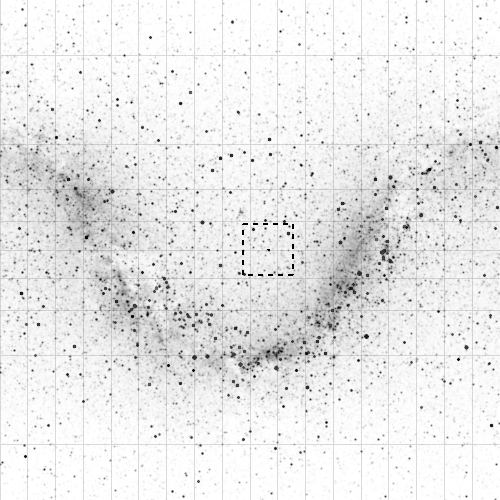
\includegraphics[width=0.31\textwidth]{ngc3521-zoom0-bw}} &
\framebox{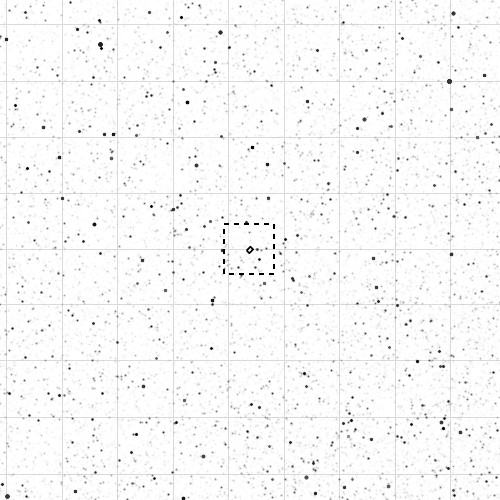
\includegraphics[width=0.31\textwidth]{ngc3521-zoom1-bw}} &
\framebox{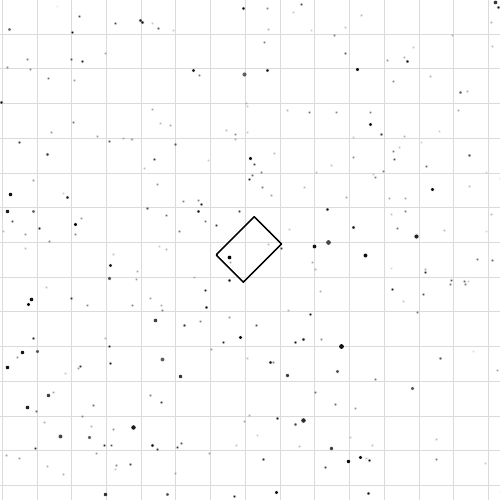
\includegraphics[width=0.31\textwidth]{ngc3521-zoom2-bw}}
\end{tabular}
\end{center}
\caption{The location of the input image on the sky.
  \captionpart{Left:} The whole sky, in Mercator projection.  The
  sinusoid-shaped feature is the Milky Way.  The dashed box shows the
  zoomed-in region.  \captionpart{Middle:} Zoomed in by a factor of
  $10$.  \captionpart{Right:} Zoomed in by a factor of $100$.  The box
  shows the outline of the input image.  These images are rendering of
  stars from the Tycho-2 catalog \cite{tycho2}.\label{fig:onthesky}}
\end{figure}


For modern astronomers, astrometric calibration is often one of the
first steps toward getting useful information out of an image of the
sky.  Aligning a new image with an \emph{astrometric reference
catalog} allows the astronomer to place the image within a standard
coordinate frame.  This allows stars, galaxies, and other objects
(\emph{sources}) in the new image to be identified with known sources,
which in turn allows astronomers to calibrate other properties of the
new image, and allows the positions of new sources to be described in
a standard reference frame.


The task of full-sky astrometric calibration---automatically finding the
astrometric calibration of an image, using only the information in the
image pixels---can be seen as a pattern recognition problem.  As
Bertin \cite{bertin2005} notes, ``astrometric and photometric
calibrations have remained the most tiresome step in the reduction of
large imaging surveys,'' so this is not only an interesting problem to
solve, but one with practical implications for astronomers.


For the purposes of astrometric calibration, we can think of the sky
as a large two-dimensional surface: the stars are very distant, so our
viewpoint is effectively fixed.  We are moving, as are the stars, but
these motions are small relative to the precision at which we
typically work.  The sky contains many stars, galaxies, and other
astronomical sources.  The stars and distant galaxies are effectively
point sources, while closer galaxies can be resolved.  Astrometric
reference catalogs list the positions, motions, and brightnesses of
these sources and serve as the ``ground truth'' or database of known
(reference) objects.  The USNO-B1 catalog \cite{usnob, nomad}, for
example, lists over one billion objects.  As many as a few percent of
these are false detections or other artifacts \cite{barroncleaning},
and some objects that should be visible are missing.


Extra sources can be due to planets, comets, satellites, or aircraft.
Missing or poorly localized source can be due to imperfections in the
imaging sensor, saturation, cosmic ray interference, or (rarely)
occlusion.  Errors in the image processing that detects sources can
lead to sources being gained or lost.  We call sources that appear in
only the input image or reference catalog \emph{distractors} and
\emph{dropouts}, respectively.  The existence of distractors and
dropouts means that we can never assume that all the objects in the
reference catalog will be contained in an image to be recognized, or
vice versa.


The images to be recognized are subregions of the sky.  Image sizes
range from nearly half the celestial sphere down to $10^{-7}$ of the
area and smaller.  The input images measure unknown bands of the
electromagnetic spectrum, and various nonlinear functions may have
been applied to the pixel values.  We cannot rely on absolute
brightness or color to recognize individual stars or galaxies.  At
best we can hope that there is some positive correlation in the
relative brightness ordering of objects in the image and the
corresponding objects in our catalog.


Astrometric calibration is an ideal task for exploring geometric
ideas in pattern recognition.  Most celestial objects are effectively
point sources, and can be found and localized to sub-pixel accuracy
using relatively simple image-processing procedures.  But since the
individual features are characterized only by their positions and
brightnesses, we must examine collections of features in order to
build distinctive patterns.  In \chapref{chap:techreport} we present
\an, which applies the geometric hashing framework to the task of
astrometric calibration.  An example of our results in shown in
\figs \ref{fig:redgreen} and \ref{fig:onthesky}.


\section{Related work in astrometric calibration}

There seem to be two distinct groups of researchers who have worked on
astrometric calibration.  The first are professional astronomers,
whose images are typically of small angular extent, long exposure
time, and high quality.  They typically assume that there is a good
initial guess of the astrometric calibration and the goal is to
produce a very accurate calibration, including image distortion.  The
second group of researchers are spacecraft engineers who want to use
the stars to estimate the attitude of a camera attached to a
spacecraft.  Here the images are of wide angular extent, have short
exposure time, and are very noisy.  Primary concerns include weight,
power consumption, and robustness (especially in avoiding false
positives), while a high degree of accuracy is neither required nor
possible given the hardware.

\subsection{Ballpark astrometric calibration}

``Ballpark'' astrometric calibration (as opposed to ``full-sky'')
requires that an initial estimate of the calibration to be provided.
Groth \cite{groth1986} presents an algorithm for matching two lists of
coordinates (eg, image coordinates in pixels and reference star
coordinates on the celestial sphere), assuming that the lists contain
a significant proportion of objects in common.  With the limited
computing resources available at the time, he suggests taking the
brightest 20 or 30 objects in each list.


Once the two lists of objects have been compiled and the brightest
objects selected, all sets of three objects are enumerated and the
triangles they form are described by a scale-, rotation-, and
translation-invariant descriptor, composed of the length ratio of the
longest to shortest edges, plus the cosine between these edges and the
\emph{sense} or \emph{parity} of the triangle.  The tolerances
associated with these features are computed (by propagating their
positional errors through the feature descriptor process) and stored,
along with the logarithm of the triangle's perimeter.  Triangles with
large length ratio are rejected since they are relatively
indistinctive.


After triangle features are extracted from both point lists, feature
matching is performed by checking whether the distance between each
pair of features is less than their corresponding tolerances.  This
process is accelerated by sorting the features on one of the feature
dimensions.  If multiple matches are found for a particular feature,
only the closest is considered.  After all the features have been
compared, many correct matches should be found, along with some false
matches.  For each match, the difference of the log-perimeters of the
two triangles is computed.  This gives the relative scales of the two
triangles and hence their coordinate frames, assuming the match is
correct.  False matches are rejected by iterative outlier detection:
the mean difference of log-perimeters is computed and matches far from
the mean are rejected.


This approach is essentially an application of the geometric hashing
method, though instead of using hashing to accelerate feature
matching, the features are simply kept in lists that are sorted on one
dimension.  Much of the subsequent work in this area follows
essentially the same path (eg, \cite{valdes1995}, \cite{dong2006}).


P\'al and Bakos \cite{pal2006} adapt the triangle-matching approach to
images containing many more objects (of order $10^4$).  Since it would
become prohibitively expensive to enumerate all triangles in such an
image, they reduce the number of triangles created by using only the
triangles created by a Delauney triangulation.  This vastly reduces
the number of triangles created, but makes the algorithm more
sensitive to dropout and distractor stars: a single extra star causes
a completely disjoint set of triangles to be created in its
neighbourhood.  To compensate for this shortcoming, they define an
\emph{extended Delauney triangulation}: for each point, they select
all points at distance $\ell$ in the Delauney triangulation, and
triangulate this set.  This process is repeated for each point.  The
first extended triangulation ($\ell = 2$) skips over the nearest set
of stars and builds larger triangles by using the next-further set of
stars.  The intent is that if some of the nearby stars are distractors
that they will be ignored when the extended triangulations are used.

\begin{figure}
\begin{center}
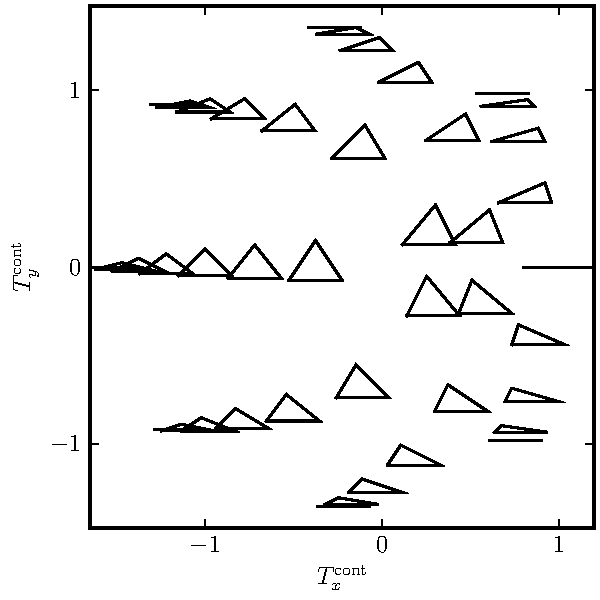
\includegraphics[width=\figunit]{pal-bakos}
\end{center}
\caption{The triangle parameterization used by P\'al and Bakos
  \cite{pal2006}.\label{pal}}
\end{figure}

P\'al and Bakos introduce a new triangle parameterization which is
continuous and sensitive to chirality (parity); see \figref{pal}.
This two-dimensional parameter space is used as the geometric feature
space.  When matching triangles between the two images, they demand a
\emph{symmetric point match}: each triangle must be the other
triangle's nearest neighbour in feature space.  Matching two images is
done by creating the lists of triangles and attempting to find
symmetric point matches.  This process is accelerated by sorting each
list by one of the coordinates.  Each triangle match is considered to
be a vote for the correspondence of the three pairs of points
composing the triangles.  These votes are accumulated in a sparse
matrix where element $(i, j)$ contains the number of votes for a
correspondence between object $i$ in the first image and object $j$ in
the second image.  After all matches are considered, the top 40\% of
the nonzero matrix elements are assumed to contain the true
correspondences.  A transformation based on these correspondences is
computed and the unitarity of the transformation matrix is used to
judge whether the match is true or false.


A different approach is taken by Kaiser \etal \cite{kaiser1999}.  They
assume they are given two lists of source positions that differ by a
rigid transformation involving scaling, rotation, and translation.  In
each image, they iterate over each pair of points and compute the
vector difference of their positions.  For each list, the log-length
and angle of the pairwise difference vectors are accumulated in a
two-dimensional histogram.  Observe that if the whole list of points
is scaled up by a constant factor, then the log-distance between each
pair of points increases by a constant amount.  Similarly, if the
whole list is rotated then the angles shift by a constant amount.
Once the two histograms have been computed, their cross-correlation is
computed.  If the two lists contain a significant number of
corresponding points, the cross-correlation signal will be strongest
at a shift corresponding to the difference in log-scale and rotation
between the lists.  This process is similar to a Hough transform
\cite{duda1972,ballard1981}, except that instead of finding the peak
of a single parameter-space histogram, we are searching for a peak in
the similarity of two histograms as we shift them with respect to each
other in parameter space.


Once the scaling and rotation between the lists has been found, the
translation can be found by scaling and rotating one of the lists into
the frame of the other list, then histogramming the vector difference
between points across the two lists.  This is a standard (generalized)
Hough transform.


\subsection{Full-sky astrometric calibration}


The majority of previous work on full-sky astrometric calibration is
motivated by the problem of spacecraft attitude estimation.  Sometimes
called the ``lost in space'' or ``stellar gyroscope'' problem, the
task is to estimate the pose of a spacecraft by using an image of the
sky captured by an onboard camera.  Although similar in general
spirit, the requirements and limitations of this application are quite
different than astronomical applications.  Mass, power consumption,
and robustness of the system are primary concerns, and as a result the
optical designs are very different from science-grade astronomical
instruments, and the available processor and memory resources are very
restricted.  Typical fields of view are tens of degrees across, and
the exposure time is kept short to allow the system to function while
the spacecraft is rotating.  As a result, image quality is typically
quite poor: often only a handful of the brightest stars are visible.
Since the field of view is large, a reference catalog of a few
thousand stars is sufficient to ensure that any view of the sky
contains many reference stars.  Since the system will only process
images from a single camera, the whole system can be customized and
calibrated to that camera.  For example, the nonlinear distortions of
the optical system can be measured, and the scale and bandpass of the
imaging system are known, so the reference catalog can be tailored to
match.


For example, Liebe \etal \cite{liebe2004} describe a system design
with a $56~\deg$ field of view and exposure time of $50~\unit{ms}$.
The resulting images contain tens of stars if the spacecraft is not
rotating, but on average only three stars will be detectable when the
rotation rate is $50~\deg/\unit{sec}$.  The paper does not describe a
particular algorithm for star identification, with the implication
that it is not a particularly difficult problem since absolute
brightness information will be available, and the total number of
stars that are visible to the camera is only a few hundred.


In earlier work \cite{liebe1993}, Liebe describes a star
identification system.  The reference catalog is composed of the $1539$
brightest stars, with brightness calibrated to the camera used in the
system.  The field of view is $30~\degrees$, and the system uses a
feature-matching approach, using the brightest star in the field and
its two nearest neighbours to define a geometric feature.  The feature
descriptor is composed of the distance from the brightest star to its
nearest and second-nearest neighbours, along with the angle between
these neighbours.  Note that this feature is not scale-invariant:
the system is only meant to recognize images taken by one camera,
so the scale is known.  An index is constructed by enumerating all
such features that could possibly be detected, given the detection
limits of the camera.  These features are coarsely quantized and
stored in a table.  To account for noise in the feature descriptors,
all neighbouring cells in the quantized feature space are also stored
in the table.  This generates $185,000$ features.  At test time, the
features in the image are enumerated and the table of features is
scanned; an exact feature match in the quantized space is assumed to
be correct.


This approach is a fairly straightforward geometric hashing technique,
except that it does not use hashing as such, and there is no voting or
verification scheme because feature aliasing is assumed not to happen.

\begin{figure}
\begin{center}
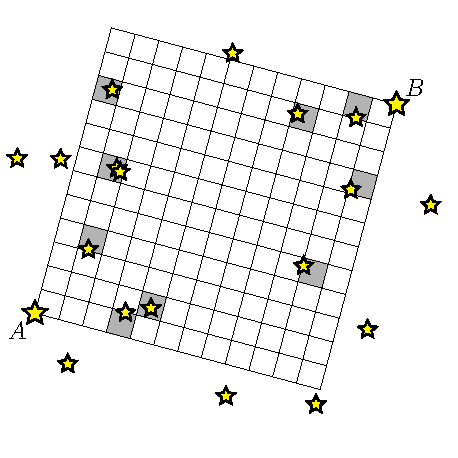
\includegraphics[width=\gridfigwidth]{grid-fig}
\end{center}
\caption{A grid-based feature: two sources (labelled $\starA$ and
  $\starB$ here) are used to define a local coordinate system which is
  discretized into a grid of cells.  Each cell becomes a bit in the
  feature descriptor; if a cell is occupied by a star its bit is set.
  This figure is inspired by MacKay \& Roweis \cite{mackay2005}.}
\label{gridbased}
\end{figure}

In contrast to systems that build features from the precise locations
of a small number of stars, Padgett and Kreutz-Delgado
\cite{padgett1997} present an approach that incorporates information
from a large portion of the image.  Their grid-based feature is
defined by first choosing one star as the reference star to define the
center of the grid, then selecting its nearest neighbour (outside an
exclusion radius) to define the orientation of the grid.  Once the
center and orientation are determined, a grid is defined, and each
remaining stars in the image is assigned to a grid cell.  The feature
is a bit vector, one bit per grid cell, where the bit is set only if
the cell contains a star.  See \figref{gridbased}.


The index is constructed by scanning the sky and selecting, for each
field of view, the $n$ brightest stars.  For each of these stars a
feature is computed and stored.  At test time, they examine the
brightest $c n$ stars (for some safety factor $c$), computing the
feature for each one and searching the index for a match.  A pair of
features is defined to match if their dot product is above a
threshold.  This is equivalent to taking the bitwise \textsc{AND} of
the bit vectors and counting the number of bits that are set.  This
search can be implemented efficiently by using lookup tables: for each
bit, they maintain a list of the features for which that bit is set.
Note that this is equivalent to using a grid-based geometric hashing
approach: each grid cell is equivalent to a discretized relative
coordinate vector, which becomes a hash key, and the ``lookup table''
is a hash table.  After all the features in the test image have been
extracted and matched to the index, the algorithm proceeds to a voting
(or perhaps ``consensus'') phase where it rejects matches that propose
a field of view that does not overlap that of the majority.


The system is designed to operate on images of diameter $8~\degrees$,
and performs well on simulated data.  They use a grid size of $40
\times 40$, and find that on average $25$ grid cells are filled.
Their index contains $13,000$ patterns, which means that false
positives are quite rare.  However, misidentification of the nearest
neighbour, or edge effects (assigning a star to the wrong grid cell
due to positional noise) mean that failures to find a match are not
uncommon, and are more likely in regions of the sky with high stellar
density.

In later work, Clouse and Padgett \cite{clouse2000} extend this
approach by using Bayesian decision theory instead of a simple
threshold on the dot product to define how well features match.  This
extension, along with smaller noise levels in the (simulated) imaging
system, allows them to extend the approach down to fields of view
$2~\degrees$ in diameter.

\comment{
  Given two features, they compute the dot product between the bit
  vectors, then proceed to estimate the probabilities that the match is
  a true positive and false positive.  These probability distributions
  are quite complex, so several simplifying approximations are made, and
  the remaining parameters are estimated by running simulations.
  }

Harvey \cite{harvey2004} presents two different approaches, one
grid-based and the other shape-based.  The grid-based approach is
similar to the Padgett--Kreutz-Delgado and Clouse--Padgett approaches
\cite{padgett1997, clouse2000}.  A coarser grid is used, so more stars
are likely to appear in each bin.  To compensate, a grid cell is only
considered ``occupied'' if it contains more than some threshold number
of stars.  The other major change is that he expects a test image to
be an ``overexposure'' or ``underexposure'' relative to the reference
catalog.  This implies that the test image should contain either a
subset or a superset of the stars in the index, and therefore the
image feature vector must be either greater than or less than an index
feature at each bit.  This allows simple bit operations to be used to
find feature matches, and feature matching is performed by a linear
scan through the index.

Harvey's shape-based approach uses constrained $n$-star constellations
in order to aggregate information from a large number of stars without
allowing the number of potential features to grow combinatorially.
Specifically, Harvey uses a pair of stars to define a narrow wedge in
the image, then describes the relative positions and angles of a fixed
number of nearby stars within that wedge.  Unfortunately, this makes
the feature highly sensitive to distractor and dropout stars, since
the feature depends on the stars in the feature being enumerated in a
particular order.  As a result, all potential features (allowing any
combination of stars to drop out) must be checked; the number of
features grows exponentially as the density of stars increases.


Harvey makes the useful observation that a cascade of indices can be
built, where each index is designed to recognize images with a particular
range of scales.


MacKay and Roweis \cite{mackay2005} point out that a grid-based
feature such as that used by Harvey leads naturally to a hashing-based
strategy.  Each grid cell is associated with a bit that is turned on
if the cell is occupied.  This value is placed in a hash table with a
mapping back to its position on the sky.  Since false positives can
occur as a result of feature aliasing or hash collision, a voting
scheme is employed: several feature matches must accumulate before the
match is accepted.  Since false negatives can occur as a result of
dropouts and distractors (\emph{any} missing or extra star causes the
hash code to change completely), many features must be extracted for
each region of the sky.


\subsection{Fine-tuning astrometric calibrations}

In order to ``co-add'' or ``stack'' astronomical images (combine
pixels from different images to produce a higher signal-to-noise
image), or to do proper-motion studies (measure the movement of stars
over time), it is necessary to fine-tune the astrometric calibration
of the images.  This is similar to the \emph{bundle adjustment}
problem in computer vision \cite{triggs2000}, in that it involves the
simultaneous optimization of the various camera and telescope
parameters and the estimated positions of objects in the world.
Fine-tuning astrometric calibrations is easier because it is
essentially two-dimensional, but more difficult because the camera
parameters include polynomial distortion terms to model the image
distortion introduced by telescope optics.


The software package \scamp by Bertin \cite{bertin2005} is a popular
tool used by astronomers to fine-tune simultaneously the astrometric
calibrations of a large collection of images.  For each image, it is
assumed that the center of the image is known to about 25\% of the
size of the image, and the scale is known to within a factor of two.
The histogram-alignment method of \cite{kaiser1999} is used to find
the translation, scaling, and rotation between the image and a
reference catalog, which allows the correspondences between image and
reference catalog stars to be determined.

The core of the \scamp system is a chi-squared minimization of the
total weighted distance between the projected positions of all star
correspondences among the set of images and the reference catalog.
The parameters to be adjusted are the center, scale, rotation, and
polynomial distortion coefficients of each image.  A key feature is
the ability to share image distortion parameters among subsets of the
images, since images taken with the same telescope are expected to
share some distortion terms due to the telescope optics.  This reduces
the degrees of freedom of the fitting process, resulting in more
robust fits.  \scamp can fine-tune thousands of images to sub-pixel
accuracy.


\section{Summary}


The task of automatically finding the astrometric calibration of an
astronomical image---this is, recognizing the stars in the image, or
locating the image on the sky---is ideal for a geometric hashing-based
approach.  Geometric hashing (or more generally, geometric feature
matching) is a widely-applicable technique for problems in which it is
desirable to build distinctive geometric features out of simple
interest-point features.  The approach is ideally suited to the
astrometric calibration problem, since images of celestial objects can
be localized to sub-pixel accuracy but have few other distinguishing
features.  Indeed, much of the previous work in ``full-sky'' and ``ballpark''
astrometric calibration can be placed within a geometric feature
matching framework.


